Encuentra el valor de la incógnita en el triángulo de la figura \ref{fig:angle_triangle_15}.

\begin{minipage}[t][5.5cm][b]{0.3\textwidth}
    \begin{figure}[H]
        \centering
        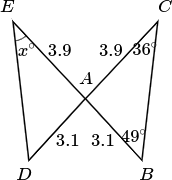
\includegraphics[width=0.8\linewidth]{../images/angle_triangle_15}
        \caption{}
        \label{fig:angle_triangle_15}
    \end{figure}
\end{minipage}\hfill
\begin{minipage}[t]{0.65\textwidth}
    \begin{solutionbox}{5.5cm}
        $\angle DAE$ forma un ángulo opuesto por el vértice con $\angle BAC$.
        \[\Rightarrow \angle DAE = \angle BAC \]
        $\triangle ABC$ y $\triangle ADE$ también tienen dos lados iguales.
        \[\therefore \triangle ABC \cong \triangle ADE\]
        Los triángulos congruentes también tienen ángulos congruentes (iguales).
        Observamos que el ángulo $x$ corresponde al
        $\angle BAC$ y $\angle BAC$ mide
        36$^\circ$.
        \[\therefore x=36^\circ\]
    \end{solutionbox}
\end{minipage}
